\section{More realistic bow shock models}
\label{sec:more-realistic-bow}

\begin{figure}
  (a)\\
  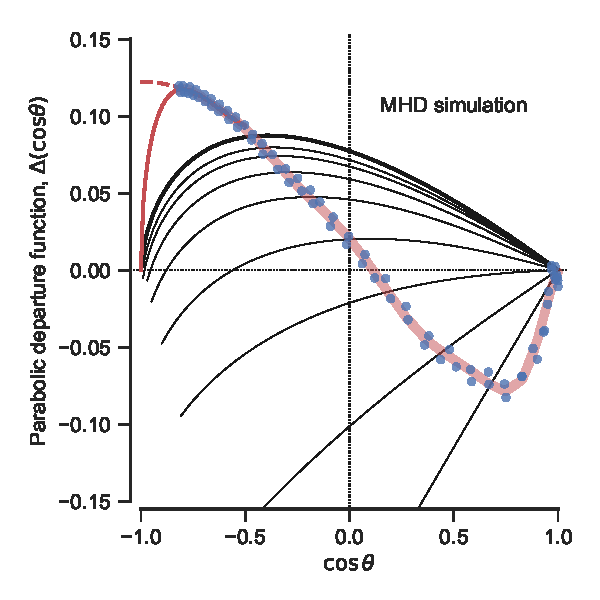
\includegraphics[width=\linewidth]
  {figs/depart-cheby-M17-MHD2040-AllB7}\\[-\baselineskip]
  (b)\\
  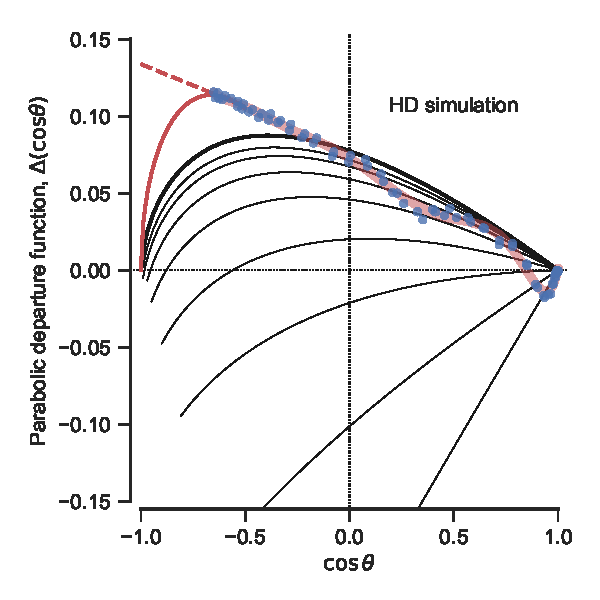
\includegraphics[width=\linewidth]
  {figs/depart-cheby-M17-HD2040}\\[-\baselineskip]
  \caption[]{Departure function for the shape of the contact
    discontinuity, measured from two numerical simulations of a
    \(20\,M_\odot\) main-sequence star, moving at \SI{40}{km.s^{-1}}
    through a uniform medium of density \SI{0.57}{cm^{-3}}
    \citep{Meyer:2017a}. (a)~Magnetohydrodynamic simulation with
    ambient magnetic field of strength \SI{7}{\micro G}, oriented
    parallel to the stellar velocity. (b)~Hydrodynamic simulation with
    zero magnetic field.  Blue dots show the measured shape, while the
    thick, pale-red line shows a 12th-order Chebyshev polynomial fit.
    The published shapes only extend to
    \(\theta \approx 130\)--\(150^\circ\), so we extrapolate the shapes out to
    \(\theta = 180^\circ\). Two different extrapolations are shown,
    corresponding to bows that are asymptotically closed (dashed red
    line) or open (solid red line).  For comparison, black lines show
    the departure function for wilkinoid (thick line) and cantoids
    (thin lines).}
  \label{fig:sim-depart}
\end{figure}

The assumptions underlying the models of the previous section may
break down in various ways.  To test whether 


Most importantly, the shocked shell may not be thin.  

\begin{figure}
  \centering
  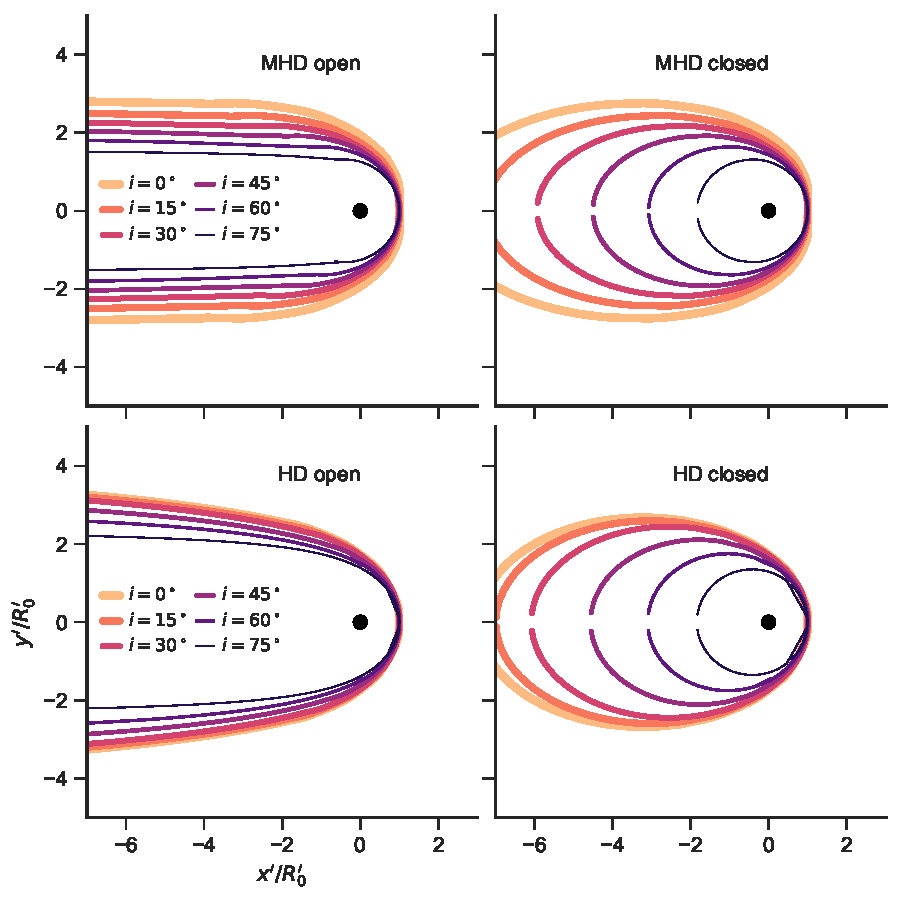
\includegraphics[width=\linewidth]{figs/test_xyprime_simulation}
  \caption[]{Projected shapes of contact discontinuity from
    simulations at different inclinations \(\abs{i}\) (varying line
    color and thickness, see key).  Top row shows magnetized
    simulation of Fig.~\ref{fig:sim-depart}a, bottom row shows
    non-magnetized simulation of Fig.~\ref{fig:sim-depart}b.  Left
    column shows asymptotically open extrapolation, right column shows
    asymptotically closed extrapolation.  All shapes are normalized to
    the projected apex distance, \(R_0'\) }
  \label{fig:sim-xyp}
\end{figure}

\begin{figure}
  \centering
  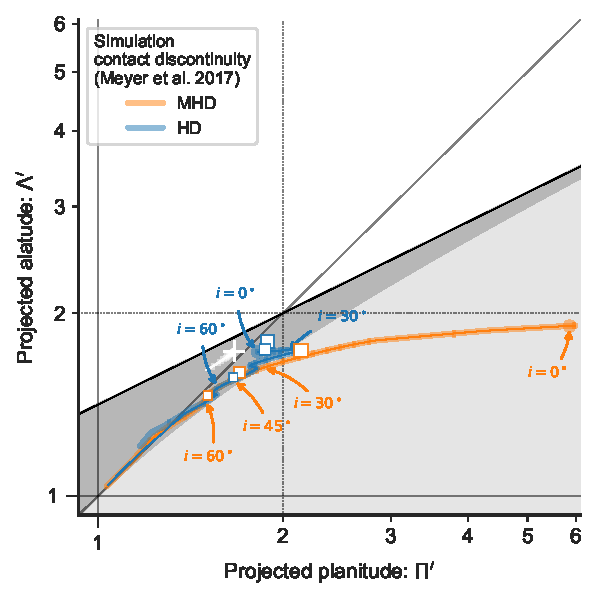
\includegraphics[width=\linewidth]{figs/m17-planitude-alatude}
  \caption[]{Apparent projected shapes of simulations.}
  \label{fig:sim-Pi-Lambda}
\end{figure}

\begin{figure}
  \centering
  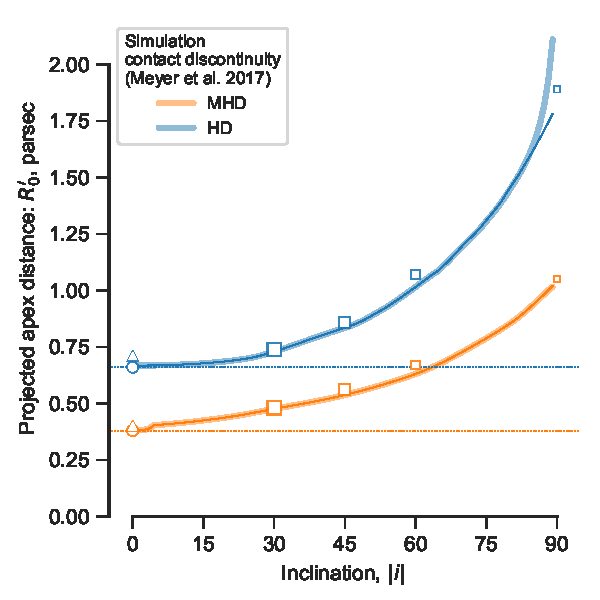
\includegraphics[width=\linewidth]{figs/m17-r0-prime}
  \caption[]{Apparent projected apex distance of simulations.}
  \label{fig:sim-R0-prime}
\end{figure}


\section{Summary and discussion}
\label{sec:conc}

We have shown that the shapes of stellar bow shocks can be usefully
characterized by two dimensionless numbers: the \textit{planitude},
\(\Pi\), or flatness of the bow's apex, and the \textit{alatude},
\(\Lambda\), or openness of the bow's wings.  The planitude and alatude can
be estimated from ratios of lengths that can be straightforwardly
measured from observations or theoretical models.  We develop a
general method for finding the projected shape,
\((\Pi', \Lambda')\), of a bow shock's limb-brightened edge, or
\textit{tangent line}, as a function of inclination angle, \(i\),
where the emission shell is idealized as a cylindrically symmetric
surface.

We first apply this method to find inclination-dependent tracks
on the projected planitude--alatude plane for the special case of
\textit{quadric} surfaces, such as hyperboloids, paraboloids, and
spheroids, where the tangent line is a conic section.  The spheroids
and hyperboloids occupy distinct regions of the plane, with the
paraboloids defining the boundary between the two.  As the inclination
is increased from \(\abs{i} = 0\) (side-on) to \(\abs{i} = 90^\circ\)
(end-on), the tracks first tend to approach the diagonal
\(\Lambda' = \Pi'\), corresponding to confocal conics, always remaining within
their own region.  At the highest inclinations, the spheroids all
converge at \(\abs{i} = 90^\circ\) on the point
\((\Pi', \Lambda') = (1, 1)\) and the paraboloids on the point
\((\Pi', \Lambda') = (2, 2)\).  The hyperboloids, on the other hand diverge as
\((\Pi', \Lambda') \to (\infty, \infty)\) for a finite
\(i_{\mathrm{crit}}\), which depends on the asymptotic opening angle
of the tail.  For \(\abs{i} > i_{\mathrm{crit}}\), the tangent line no
longer exists for the hyperbola, and it no would longer appear to be a
bow shock.

We then apply the projection method to a set of thin-shell
hydrodynamic models of bow shocks: the \textit{wilkinoid} from a
wind-parallel stream interaction and the \textit{cantoids} from
wind-wind interactions.  We generalize the latter to the
\textit{ancantoids}, where one of the winds is anisotropic.  We find
that the wilkinoid is confined to a small region of the
\(\Pi'\)--\(\Lambda'\) plane, with projected planitude and alatude varying with
inclination by \(< 15\%\).  The cantoids and ancantoids with
sufficiently small values of \(\beta\), the wind momentum ratio, have more
interesting behavior, with tracks that pass from the spheroid region
at low inclinations to the hyperboloid region at high inclinations.  

This paper is the first of a series that will apply our shape analysis
to a wide variety of models and observations of stellar bow shocks.
In a second paper \citep{Henney:2018a}, we consider the alternative
model of dusty radiation-driven bow wave, instead of a hydrodynamic
bow shock, and also calculate the signature in the planitude--alatude
plane of oscillations in the bow shape, which may be due to
instabilities or a time-varying source.  In a third paper
\citep{Henney:2018b}, we apply our techniques to observational
datasets for three different classes of stellar bow shocks: OB stars,
cool giants/supergiants, and young stars in the extended Orion Nebula.
In a fourth paper \citep{Tarango-Yong:2018b}, we analyze the proplyd
bow shocks in the core of the Orion Nebula.


%and was applied to the proplyds in the core of the ONC.
%We started measuring the projected characteristic radii $(R'_0,R'_c)$ for each proplyd in our
%sample and compare them with the ``conic equivalent'' of a two winds interaction model based 
%on \CRW{} work to estimate the intrinsic bow shock shape and get the ionizing flux for ionization balance 
%and the stagnation pressure for our sample of proplyds.
%Most results are consistent with a proplyd's photoevaporated flow with an anisotropic density
%distribution, with different anisotropy degrees. We ound that LV4 has the least anisotropic flow,
%while LV2 has the most anisotropic flow. And for the 177-341, 169-348 and 180-331 we found out that 
%the stellar wind is not enough to keep their bow socks stationary.

%%% Local Variables:
%%% mode: latex
%%% TeX-master: "quadrics-bowshock"
%%% End:
